%% Journal submission draft.
%%
%% Status: complete except Section 4.7, which reports the language-model arms
%% and is blocked on the credential decision. Everything else is written against
%% numbers in ../results.json, checked by ../claims.py.
%%
%% Build:  pdflatex paper && bibtex paper && pdflatex paper && pdflatex paper

\documentclass[preprint,12pt]{elsarticle}

\usepackage{amsmath,amssymb}
\usepackage{graphicx}
\usepackage{booktabs}
\usepackage{url}
\usepackage[T1]{fontenc}
\usepackage{xcolor}
\usepackage{hyperref}
\hypersetup{colorlinks=true,linkcolor=blue,citecolor=blue,urlcolor=blue}
\graphicspath{{../figures/}{figures/}}

\journal{[see cover letter]}

\begin{document}

\begin{frontmatter}

\title{What a monitoring agent is entitled to conclude: identifiability limits
for fault diagnosis in laser powder bed fusion}

\author[a]{Soham Jain\corref{cor1}}
\ead{f20240343@pilani.bits-pilani.ac.in}
\cortext[cor1]{Corresponding author.}
\author[a]{Tribeni Roy}
\affiliation[a]{organization={Department of Mechanical Engineering,
                Birla Institute of Technology and Science Pilani},
                city={Pilani}, country={India}}

\begin{abstract}
In-situ monitoring is standard on metal additive manufacturing systems, and
software that reads those signals and names a process cause is now being built
on top of it. This paper asks what such a system is entitled to claim. Treating
diagnosis as a hypothesis test on a calibrated thermal model, and profiling out
the unknown fault severity, yields for each candidate cause a residual
distributed as chi-squared on $S-1$ degrees of freedom. The set of causes not
rejected at level $\alpha$ is then a confidence set that contains the true cause
with probability exactly $1-\alpha$, with no prior and no training data. We call
it the certificate, and it is the object a diagnostic agent may report.

Three results follow. The separation floor used in the diagnosability literature
is not a convention but an unstated assumption about signal strength: a pair of
causes at mutual angle $\Delta$ is resolvable only if
$\Delta > 2\arcsin(\sqrt{q_{1-\alpha}}/\rho)$, so a ten degree floor asserts a
whitened signal-to-noise ratio of 28.1. Second, for a three-instrument coaxial
suite reading one instant, the certificate names a unique cause in 3.5\,\% of
builds at that signal strength, and a maximum-likelihood estimator working from
the same physical model and the same data recovers the true cause 44.0\,\% of
the time; regressing the same signals on build context the machine already
records raises the unique-cause rate to 95.3\,\%. Third, writing the Jacobian as
$J = MC$, where $C$ carries the faults into four physical channels and $M$
carries the channels into the instruments, shows
$C[:,\mathrm{power}] = -C[:,\mathrm{gas}]$ exactly, so laser power and shielding
gas are confounded for every instrument set at every operating point and in any
stack of operating points. Deliberate probing cannot reach them, and the best
two-point probe leaves the next-worst pair at $6.1^\circ$, short of the floor.
What separates them is not richer observation but the fact that the two vary
differently across a build.
\end{abstract}

\begin{keyword}
laser powder bed fusion \sep in-situ monitoring \sep diagnosability \sep
identifiability \sep set-valued prediction \sep digital twin
\end{keyword}

\end{frontmatter}

%% ===========================================================================
\section{Introduction}
\label{sec:intro}

A laser powder bed fusion machine carries instruments that watch the melt pool
while it builds: a coaxial photodiode integrating thermal emission, a camera
reporting melt pool extent, sometimes a pyrometer inferring temperature. A large
literature maps those signals onto defects and reports high accuracies. A newer
body of work puts software on top that reads the same signals and tells an
operator what went wrong, often phrased as a digital twin with an agent attached
\cite{Chen2025}.

Such a system makes a claim of a particular kind. Saying that a build suffered a
power fault rather than a shielding gas fault is a statement about causes, not
about outcomes, and the data may not support it. The two faults can produce melt
pool signatures that differ by less than the measurement noise, and where that
happens no classifier, no volume of training data and no language model
separates them. The limit is in the physics of how the faults reach the
instruments, not in the algorithm reading them.

This is not the question the monitoring literature has been answering. Of
nineteen studies extracted for this work, eighteen perform in-situ monitoring,
seven classify an outcome such as porosity or a geometric defect
\cite{Scime2019,Bugatti2022}, three estimate a process input from the signal
\cite{Blanc2024,Reijonen2024,kNN2025}, one of those three only as a lumped group
rather than separately \cite{kNN2025}, and \emph{none} analyses whether the
causes it names are separable in principle. The accuracy figures are real; they
simply answer a different question from the one a diagnostic claim poses.

We supply the missing layer. Section~\ref{sec:method} develops a test: profile
out the unknown fault severity, and what remains for each candidate cause is a
residual with an exact chi-squared reference distribution. The causes that
survive form a confidence set, which we call the certificate, containing the
true cause with probability exactly $1-\alpha$. It is cheap, it needs no
training data and no prior over fault frequencies, and it is the set a
diagnostic agent is entitled to report. Reporting one member of a four-member
certificate is not a confident answer; it is an unsupported one.

\paragraph{Contributions}
\begin{enumerate}
\item A certificate for cause attribution in laser powder bed fusion, with
exact finite-sample coverage, built on a calibrated thermal model rather than on
labelled data (Section~\ref{sec:test}), and a demonstration that building it on
the model's tangent rather than the model itself makes it exclude the true cause
(Section~\ref{sec:exact}).
\item A derivation of the separation floor used in diagnosability analysis from
the test, showing it to be an assumption about signal-to-noise rather than a
convention, and pricing every fault pair in the signal and the fault magnitude
it would need (Sections~\ref{sec:floor} and \ref{sec:priced}).
\item A measurement of what a standard coaxial suite licenses: unique
attribution in 3.5\,\% of builds at one instant against 95.3\,\% with build
context, and the equivalence structure in between
(Sections~\ref{sec:size} and \ref{sec:classes}).
\item A factorisation of the Jacobian through four physical channels that makes
the power-against-gas degeneracy a theorem rather than a numerical finding, and
a negative result on active probing that follows from it
(Section~\ref{sec:probe}).
\item A benchmark, with its prompts and scoring defined against the certificate
rather than against the truth, for measuring how often a diagnostic agent claims
more than the data supports (Sections~\ref{sec:agents} and \ref{sec:arms}).
\end{enumerate}

%% ===========================================================================
\section{Related work}
\label{sec:related}

\subsection{What in-situ monitoring reports}

Melt pool monitoring signals have been mapped to flaw formation with supervised
learning \cite{Scime2019}, to geometric and surface defects through recoater
imaging \cite{Bugatti2022}, and to local powder layer thickness through infrared
thermography \cite{Liu2022}. A smaller group estimates process inputs rather
than outcomes: from on-axis video \cite{Blanc2024}, from photodiode response to
laser parameters and gas flow \cite{Reijonen2024}, and from melt pool images by
nearest neighbours \cite{kNN2025}. Spatial variation in coaxial signals across a
build has been modelled explicitly \cite{Raj2023}, which matters here because
that variation is what Section~\ref{sec:priced} shows to be the only thing
separating two of the faults.

Sensor placement for fault diagnosis has a long structural tradition
\cite{Krysander2008}, which asks which faults an equation set can distinguish
given which measurements. That tradition supplies the question this paper asks
of a melt pool, and our certificate is its quantitative counterpart at a stated
noise level.

\subsection{Reporting a set instead of an answer}

Answering with a set rather than a point, or declining to answer, is old. Chow
established the optimal error-reject tradeoff for pattern recognition
\cite{Chow1970}. Conformal prediction gives distribution-free prediction sets
with finite-sample coverage for any underlying model \cite{Angelopoulos2023}.

Our certificate shares the set-valued output and the coverage guarantee, and
differs in where the guarantee comes from. Conformal prediction is calibrated on
held-out data and makes no use of a physical model; the certificate is
calibrated by the reference distribution of a profile likelihood on a model of
the process and uses no data beyond the build in front of it. For a process
where faults are rare, deliberately inducing them is expensive, and a calibrated
forward model exists, that trade is the right way round. The two are
complementary rather than competing: a conformal wrapper calibrated on real
builds would answer the same question with different assumptions, and comparing
them is worthwhile future work.

\subsection{Agents that name causes, and what they claim}

Language models report confidence that is systematically higher than their
accuracy. Verbalized uncertainty from both language and vision-language models
is overconfident \cite{Groot2024}, and vanilla verbalized confidence shows
significant overconfidence and poor failure prediction, improving only partly
under prompting strategies and not reliably with scale \cite{Xiong2023}. A
diagnostic assistant inherits that tendency, and the setting here makes it worse
rather than better: an operator asking what went wrong invites a single answer,
and the training distribution rewards giving one.

%% ===========================================================================
\section{Method}
\label{sec:method}

\subsection{Forward model, faults, and instruments}
\label{sec:forward}

The thermal model is an Eagar--Tsai solution with an analytic keyhole depth
correction, calibrated against seven single tracks from the 2022 Additive
Manufacturing Benchmark on nickel alloy 718 \cite{Weaver2024}, in the form and
at the parameter values established in the companion conference paper. Effective
absorptivity, conductivity, heat capacity and a keyhole coefficient are fixed at
their stored calibrated values throughout, so that nothing here depends on a
refit.

Five faults are considered, each entering through a stated physical route: a
laser power deviation; a scan speed error; a powder layer thickness deviation,
acting on both effective absorptivity and effective conductivity; shielding gas
degradation, acting as Beer--Lambert attenuation of the beam
\cite{Reijonen2020}; and local heat accumulation from part geometry, acting as a
preheat rise. Power and speed are fractional deviations. The other three are
dimensionless severity indices whose physical meaning comes from the coupling
constant each multiplies, so a common numerical magnitude across the five does
\emph{not} represent a common severity, and no comparison in this paper is made
at fixed magnitude.

Three instruments are read: a coaxial photodiode in radiometric power, a camera
reporting melt pool area from a liquidus threshold, and a two-colour pyrometer
at 750 and 950\,nm reporting temperature. Their relative noise is derived from
transduction rather than assumed, under the single assumption that every
radiometric channel carries the same fractional noise $\varepsilon$. The derived
set is $1 : 0.142 : 1.061$.

\subsection{The observation model, and where $\varepsilon$ goes}
\label{sec:obs}

A fault is a type $k$ and a magnitude $f$. Write
$J[s,k] = (1/y_s)\,\partial y_s/\partial f_k$ for the relative-sensitivity
Jacobian, by central differences at a step whose convergence is checked. The
relative deviation of the instruments from a healthy build is, to first order,
$z = f J[:,k]$ plus noise of standard deviation $\sigma_s \varepsilon$ on
sensor $s$. Dividing through,
%
\begin{equation}
z_w \;=\; \frac{z}{\sigma \varepsilon} \;=\; f\,J_w[:,k] + e,
\qquad e \sim \mathcal{N}(0, I_S),
\label{eq:obs}
\end{equation}
%
so $z_w$ is measured in standard deviations and $J_w = J/\sigma$ is the whitened
Jacobian on which diagnosability angles are computed.

The common noise level $\varepsilon$ never had to be named in a purely
geometric analysis, because angles between whitened columns depend on the ratios
$\sigma_s$ alone and a common factor cancels. A hypothesis test is not scale
invariant: whether an observation is consistent with a cause depends on how
large the signal is against the noise. We therefore parameterise everything by
the whitened signal-to-noise ratio
%
\begin{equation}
\rho \;=\; \|f J_w[:,k]\| \;=\; f\,\|J_w[:,k]\| \,/\, \varepsilon ,
\label{eq:rho}
\end{equation}
%
rather than by $f$ and $\varepsilon$ separately. Any pair of a magnitude and a
noise level giving the same $\rho$ behaves identically under the test, so
reporting against $\rho$ claims no absolute noise figure. Where a physical
magnitude is wanted we fix $\varepsilon = 1\,\%$ as a stated convention and
invert Equation~\eqref{eq:rho}; at that convention $\rho = 28$ is a 3.2\,\%
power deviation, a 9.4\,\% speed deviation or a preheat index of 0.43.

\subsection{The certificate}
\label{sec:test}

Nobody knows how severe a fault is, and the question is only which cause it was,
so the magnitude is a nuisance parameter and is profiled out. For candidate
cause $k$, with $u_k = J_w[:,k]/\|J_w[:,k]\|$,
%
\begin{equation}
\hat f_k = \frac{\langle z_w, J_w[:,k]\rangle}{\|J_w[:,k]\|^2},
\qquad
R_k = \bigl\| z_w - \hat f_k J_w[:,k] \bigr\|^2
    = \|z_w\|^2 - \langle z_w, u_k\rangle^2 .
\label{eq:resid}
\end{equation}
%
$R_k$ is the squared length of the part of the observation that no magnitude of
cause $k$ explains. Under the hypothesis that $k$ is the true cause,
$z_w - f J_w[:,k]$ is standard normal in $S$ dimensions and $R_k$ is its squared
projection onto the $S-1$ dimensional subspace orthogonal to $u_k$, so
%
\begin{equation}
R_k \sim \chi^2_{S-1} \quad\text{whatever } f \text{ is},
\end{equation}
%
one degree of freedom having been spent on the magnitude. The distribution is
exact rather than asymptotic and involves no prior over causes. The
\emph{certificate} is
%
\begin{equation}
C_\alpha(z) \;=\; \bigl\{\, k \;:\; R_k \le q_{1-\alpha}(S-1) \,\bigr\},
\label{eq:cert}
\end{equation}
%
the set of causes not rejected at level $\alpha$, and because the test has exact
size $\alpha$ under each hypothesis it contains the true cause with probability
exactly $1-\alpha$. An empty certificate is a legitimate outcome, occurring
about $\alpha$ of the time, and says that no single cause explains the data.

\subsection{The geometry, and the separation floor}
\label{sec:floor}

Write $\rho = \|z_w\|$ for the observed signal-to-noise and $\psi_k$ for the
angle between the observation and cause $k$'s signature direction. Then
$\langle z_w, u_k\rangle = \rho\cos\psi_k$ and Equation~\eqref{eq:resid} becomes
$R_k = \rho^2 \sin^2\psi_k$, so
%
\begin{equation}
k \in C_\alpha
\iff
\sin\psi_k \le \frac{\sqrt{q_{1-\alpha}(S-1)}}{\rho} .
\label{eq:cone}
\end{equation}
%
The certificate is a cone about the observation, of half-angle
$\psi^\ast = \arcsin(\sqrt{q}/\rho)$, and every signature direction inside it is
admissible (Fig.~\ref{fig:cone}).

Two causes at mutual angle $\Delta$ both fall inside the cone whenever the
observation lies near their bisector, so the pair is resolvable only if
%
\begin{equation}
\Delta \;>\; 2\arcsin\!\left(\frac{\sqrt{q_{1-\alpha}(S-1)}}{\rho}\right).
\label{eq:floor}
\end{equation}
%
Diagnosability studies, including our own earlier work, adopt a separation floor
of ten degrees as a practical convention. Equation~\eqref{eq:floor} shows it is
not a free choice but a statement about signal strength, and
Section~\ref{sec:floorresult} reports which.

\subsection{Whitening observations that are not independent}
\label{sec:whiten}

Whitening exists so that the geometry means separability, which requires the
noise to be isotropic afterwards. Dividing each row by its own standard
deviation achieves that only when the observations are independent. Three
instruments read at one instant are independent by assumption, so
Sections~\ref{sec:floorresult} to \ref{sec:classes} are unaffected by what
follows.

The enlarged observation of Section~\ref{sec:context} is different. Its entries
are least-squares coefficients of each sensor's residual on build regressors,
and writing $G$ for the $N \times p$ regressor matrix,
%
\begin{equation}
\hat c_s = (G^{\mathsf T}G)^{-1}G^{\mathsf T} z_s
\quad\Longrightarrow\quad
\operatorname{Cov}(\hat c_s) = \sigma_s^2 \varepsilon^2 (G^{\mathsf T}G)^{-1},
\end{equation}
%
which is not diagonal whenever the regressors are correlated. In the scan plan
used here, turn density and support depth give a coefficient correlation of
0.577. Sensors being independent, the covariance of the stacked observation is
the Kronecker product
%
\begin{equation}
\operatorname{Cov} \;=\; \varepsilon^2
\left( \operatorname{diag}(\sigma^2) \otimes (G^{\mathsf T}G)^{-1} \right),
\label{eq:kron}
\end{equation}
%
and the correct whitening is its inverse Cholesky factor, not the reciprocals of
the marginal standard errors. Using the marginal errors as though the
coefficients were independent gives a 95\,\% certificate that covers 93.8\,\% of
the time and moves the pairwise angles by up to 8.8 degrees, enough to change
which pair is worst. Equation~\eqref{eq:kron} is used throughout, and verified
against per-segment noise put through the same least squares.

\subsection{Profiling through the model rather than its tangent}
\label{sec:exact}

Equation~\eqref{eq:resid} assumes the response to a fault is a straight line
through the healthy point. The exact response is not, and the departure is a
fixed bias perpendicular to the fault's own signature, which enters the residual
as its square and consumes the test's budget. The certificate is therefore built
on the exact profile residual
%
\begin{equation}
R_k(z) \;=\; \min_{f} \;
\bigl\| z_w - g_k(f) / (\sigma\varepsilon) \bigr\|^2 ,
\label{eq:exact}
\end{equation}
%
where $g_k(f)$ is the exact relative deviation under a fault of type $k$ and
magnitude $f$. This is a profile likelihood with one nuisance parameter and so
keeps the same reference distribution. Response curves are built once, 49
forward evaluations per fault, and cached as monotone cubic interpolants;
monotone cubics rather than splines because the camera's extent comes from a
threshold, and an interpolant that can overshoot would invent features the model
does not have. Section~\ref{sec:exactresult} reports what the linearisation
would have cost.

\subsection{Build context}
\label{sec:context}

A build is thousands of segments whose toolpath, layer index, position along the
gas-flow axis and local support depth the machine knows in advance. The five
faults do not vary identically across them. Regressing each sensor's residual on
those known regressors gives, for fault $k$, an enlarged signature
$J[s,k]\,B[j,k]$, where $B = (G^{\mathsf T}G)^{-1}G^{\mathsf T}M$ carries each
fault's spatial modulation onto the regressors. The enlarged observation is 15
coefficients, three sensors by five regressors, with 14 degrees of freedom and
the covariance of Equation~\eqref{eq:kron}. Everything else in the method is
unchanged.

\subsection{Agents, prompts and scoring}
\label{sec:agents}

An agent is anything that reads an observation and returns a set of causes. Five
deterministic arms bracket the language-model ones, because a score without a
ceiling and a floor means nothing: an \emph{oracle} that names the truth; a
\emph{maximum likelihood} arm naming the single best-fitting cause, which is
what a trained classifier does; the \emph{certificate} itself; an
\emph{everything} arm naming all five; and a \emph{chance} arm naming one at
random.

The language-model arms see the nominal process conditions, the relative change
in each signal, the stated noise level and a physical description of each
candidate cause. They never see the Jacobian, the whitened geometry or the
certificate, since an agent shown those would be running the test rather than
being tested. Two prompt styles are used and reported separately: a
\emph{neutral} style asking which causes are consistent and stating that naming
several is a valid answer, and an \emph{operator} style asking what went wrong
in the build, as a monitoring dashboard would. A prompt that forces a unique
reply would make an over-attribution rate an artefact of its own wording, so the
difference between the two styles is measured rather than assumed away. A
\emph{certified} style supplies the certificate and forbids narrowing without
naming a distinguishing measurement, with the intersection enforced in code
rather than trusted to the instruction.

Scoring is defined against the certificate rather than the truth, because
accuracy is the measure that creates the problem: an agent naming one cause on a
build whose data admits four is accurate a quarter of the time by luck.

\begin{description}
\item[coverage] the truth is in the reported set.
\item[over-attribution] the agent named exactly one cause, given that the
certificate held two or more. Conditioned on ambiguity, so an agent is not
penalised for being decisive when the data is.
\item[decisiveness] the agent named exactly one cause, given that the
certificate held exactly one. Reported alongside over-attribution, which alone
has the trivial optimum of never committing.
\item[admissibility] the reported set is a subset of the certificate.
\item[unsupported exclusion] the agent left out a cause the certificate
contains. Operationally the costly error: ruling out the real cause sends an
engineer to the wrong subsystem.
\item[skill] among over-attributed cases, $(\text{accuracy} - \text{chance})/
(1 - \text{chance})$ with chance the mean of $1/|C|$ over those cases. Zero
means guessing inside the certificate; one means always right.
\end{description}

%% ===========================================================================
\section{Results}
\label{sec:results}

Unless stated otherwise, $\alpha = 0.05$, observations are generated from the
full nonlinear forward model, and cases are drawn at a target $\rho$ rather than
at a common magnitude for the reason given in Section~\ref{sec:forward}. Rates
are estimated from 1500 cases per signal level, 300 per fault, so a reported
rate near 0.05 carries a standard error of about 0.006 and one near 0.95 the
same; admissibility entries come from 3000 draws per cell, a standard error of
at most 0.009.

\subsection{The floor is an assumption about signal strength}
\label{sec:floorresult}

With three instruments, $S-1 = 2$ and $q_{0.95}(2) = 5.9915$. Inverting
Equation~\eqref{eq:floor} at $\Delta = 10^\circ$ gives $\rho = 28.08$: the ten
degree floor asserts that the whitened signal is about 28 standard deviations,
which at $\varepsilon = 1\,\%$ is a 3.2\,\% power deviation. For the enlarged
observation, with 14 degrees of freedom, the same floor corresponds to
$\rho = 55.84$.

\subsection{What the suite licenses}
\label{sec:size}

Fig.~\ref{fig:certificate} reports how often the certificate names exactly one
cause. Reading one instant, it does so in 3.5\,\% of builds at $\rho = 28$,
rising only to 24.2\,\% at $\rho = 120$, and the mean certificate holds 4.26 of
the five causes at $\rho = 28$. Regressing the same three signals on build
context, the unique-cause rate is 95.3\,\% at $\rho = 28$, which is the test's
own ceiling of $1 - \alpha$, and is already there at $\rho = 14$.

Broken out by fault at $\rho = 56$, the instantaneous unique-cause rate is
0.003 for layer, 0.007 for power, 0.010 for gas, 0.037 for speed and 0.273 for
geometry. Geometry is the only cause this suite can name, which is consistent
with its being the only one more than $3.6^\circ$ from everything else.

\subsection{The equivalence structure}
\label{sec:classes}

Fig.~\ref{fig:admissibility} shows the admissibility matrix
$A[k,l] = \Pr(l \in C_\alpha \mid \text{truth} = k)$. Its diagonal is the
coverage and is a check on the implementation rather than a result; its
off-diagonal entries say how often a wrong cause survives.

The matrix is not symmetric and is not symmetrised. A fault with a short
whitened signature produces an observation near the origin, where every
signature direction passes, so a weak cause admits strong ones more readily than
the reverse: at $\rho = 28$, geometry admits speed 83.9\,\% of the time while
speed admits geometry 60.3\,\% of the time.

Thresholding at $0.5$ and taking connected components, the instantaneous suite
has all five causes in one class up to $\rho = 56$; at $\rho = 120$ geometry
separates, leaving $\{\text{power}, \text{speed}, \text{layer}, \text{gas}\}$ as
a clique, meaning every member is confusable with every other rather than merged
through a chain. With build context there are five singletons at every signal
level from $\rho = 14$ up. Admissibility is not transitive, so connected
components are the conservative summary and the maximal cliques the optimistic
one; both are reported.

\subsection{Every pair, priced in signal and in fault magnitude}
\label{sec:priced}

Equation~\eqref{eq:floor} inverts to give the signal each pair would need
(Fig.~\ref{fig:required}), and Equation~\eqref{eq:rho} converts that into a
fault magnitude. Instantaneously, separating power from speed needs
$\rho = 398$, which at $\varepsilon = 1\,\%$ is a 46\,\% power deviation;
separating power from layer needs $\rho = 867$, a 99\,\% power deviation; layer
from gas needs a layer severity index of 2.7, where 1.0 is the convention for
severe. Those are not faults, they are different processes.

With build context every pair needs between $\rho = 11.7$ and $\rho = 22.0$. In
particular power against gas becomes resolvable at $\rho = 18.8$, a 0.2\,\%
power deviation, having been unresolvable at any signal strength whatever. That
is the sharpest statement of what the build's own known structure is worth.

\subsection{A linearised certificate rules out the true cause}
\label{sec:exactresult}

The exact response departs from its own tangent by a fixed perpendicular bias.
For a power fault at $\varepsilon = 1\,\%$ that departure is 0.19 at
$\rho = 28$, 0.77 at $\rho = 56$ and 1.72 at $\rho = 120$, the last consuming
49.6\,\% of the test's budget $q = 5.99$ on its own.

Fig.~\ref{fig:coverage} shows the consequence. Profiled through the exact model,
coverage holds at nominal across the range. Profiled through the tangent, it
falls to 0.76 by $\rho = 120$. Under-coverage is the dangerous direction: it
means the test excludes the true cause more often than advertised, so a
linearised certificate would license an agent to rule out the actual fault. The
mean certificate size is essentially unchanged between the two, so the result of
Section~\ref{sec:size} is not an artefact of linearising.

\subsection{The channel factorisation and the ceiling on probing}
\label{sec:probe}

Everything the model knows reaches the instruments through four physical
channels: absorbed power $AP$, scan speed, effective conductivity and local
preheat. The Jacobian therefore factors,
%
\begin{equation}
J \;=\; M\,C ,
\label{eq:factor}
\end{equation}
%
with $C$ of size $4 \times 5$ carrying faults into channels and $M$ of size
$3 \times 4$ carrying channels into instruments. $C$ is a property of the faults
and the material; $M$ is a property of the instruments and the operating point.
A probe changes $M$ and cannot touch $C$. Written out from the fault routes of
Section~\ref{sec:forward}, with channels in log units except preheat in kelvin,
$C$ is given in Table~\ref{tab:C}; Equation~\eqref{eq:factor} reproduces the
directly computed Jacobian to $6.8\times10^{-5}$ relative, which is the
finite-difference error.

\begin{table}[htbp]
\centering
\caption{$C$, how each fault moves each channel. A power fault raises absorbed
power and a gas fault lowers it, and neither does anything else, so the two
columns are exactly antiparallel.}
\label{tab:C}
\begin{tabular}{@{}lrrrrr@{}}
\toprule
 & power & speed & layer & gas & geometry \\
\midrule
$\ln(AP)$      & $1$ & $0$ & $-0.044$ & $-1$ & $0$ \\
$\ln(v)$       & $0$ & $1$ & $0$      & $0$  & $0$ \\
$\ln(k)$       & $0$ & $0$ & $0.5$    & $0$  & $0$ \\
$T_0$ (K)      & $0$ & $0$ & $0$      & $0$  & $100$ \\
\bottomrule
\end{tabular}
\end{table}

Since $C[:,\mathrm{power}] = -C[:,\mathrm{gas}]$ exactly, it follows that
$(MC)[:,\mathrm{power}] = -(MC)[:,\mathrm{gas}]$ for \emph{every} $M$. The two
columns are antiparallel in every instrument set, at every operating point, and
in any stack of operating points. $C$ has rank 4 and a one-dimensional null
space lying exactly along equal power and gas: such a combined fault moves no
channel, so it moves no observable that could be built. This is strictly
stronger than reporting the pair confounded for one suite at one operating
point.

Probing does not rescue the other nine pairs either (Fig.~\ref{fig:probing}).
Two well-chosen operating points raise the second-worst pair from $0.32^\circ$
to $5.95^\circ$, and the best second point over a grid search with local
refinement, 440\,W and 2.29\,m/s against a nominal 285\,W and 0.96\,m/s, reaches
$6.15^\circ$. Four points attain nominal rank 4 with a condition number of
$2.9\times10^{5}$, which is rank in name only. The mechanism is visible in $M$:
its preheat column is of order $10^{-3}$ where its absorbed-power column is of
order 1, at every operating point tested, because a kelvin of preheat barely
moves a pool running near 3000\,K. The fourth channel is intrinsically weak and
no operating point makes it otherwise.

Build context clears power against gas, which is not a contradiction and is
worth seeing clearly. Equation~\eqref{eq:factor} assumes the fault magnitudes
are the same at every epoch. Build context breaks that assumption rather than
enriching $M$: a fault's severity varies across the build along its own profile,
so what is observed is $J[s,k]B[j,k]$, and $B[:,\mathrm{power}]$ is not
proportional to $B[:,\mathrm{gas}]$ even though the channel columns are. The
escape route is differential modulation of the faults, not richer observation.
The only thing that separates a power fault from a gas fault is that the two
vary differently across a build.

\subsection{The deterministic arms}
\label{sec:arms}

Table~\ref{tab:arms} reports the five deterministic arms on 6000 instantaneous
cases, 5259 of them, or 87.65\,\%, with an ambiguous certificate. Two rows are worth
reading on their own.

A maximum-likelihood estimator, working from a perfect physical model and the
same data, recovers the true cause 44.0\,\% of the time, rising from 28.6\,\% at
$\rho = 14$ to 61.5\,\% at $\rho = 120$. That is the number the monitoring
literature would report as accuracy, produced by an estimator strictly better
than any classifier trained on the same signals. Its skill above chance inside
the certificate is 0.17: it is doing something real, and not much.

The oracle over-attributes on every ambiguous case. Being told the answer does
not make naming it supported by the data, and nothing in the table except the
certificate avoids that.

\begin{table}[htbp]
\centering
\caption{Deterministic arms, 6000 instantaneous cases, 5259 of them ambiguous.
Over-attribution is conditioned on ambiguity and decisiveness on its absence, so
the two must be read together: \emph{everything} scores a perfect zero on the
first only by never committing to anything.}
\label{tab:arms}
\begin{tabular}{@{}lrrrrr@{}}
\toprule
arm & coverage & mean $|R|$ & over-att. & decisive & skill \\
\midrule
oracle             & 1.000 & 1.00 & 1.000 & 1.000 & 1.00 \\
maximum likelihood & 0.440 & 1.00 & 1.000 & 1.000 & 0.17 \\
certificate        & 0.951 & 3.70 & 0.000 & 1.000 & --- \\
everything         & 1.000 & 5.00 & 0.000 & 0.000 & --- \\
chance             & 0.201 & 1.00 & 1.000 & 1.000 & $-0.08$ \\
\bottomrule
\end{tabular}
\end{table}

\subsection{The language-model arms}
\label{sec:llm}

\textcolor{red}{\textbf{[Pending.]} This section reports the unconstrained and
certified language-model arms under both prompt styles, against the brackets of
Table~\ref{tab:arms}. The harness, prompts, parser and scoring are complete and
tested; the runs are outstanding.}

%% ===========================================================================
\section{Discussion}
\label{sec:discussion}

\subsection{What this means for a monitoring claim}

A reported accuracy for cause attribution is uninterpretable without the
certificate size that goes with it. On the suite studied here, a classifier
reporting 44\,\% accuracy at one instant and one reporting 95\,\% with build
context are not two algorithms of different quality; they are the same question
asked where the data answers it and where it does not. The useful artefact to
publish alongside a monitoring result is therefore not a confusion matrix but
the admissibility matrix of Fig.~\ref{fig:admissibility}, which says what the
confusion matrix could have looked like at best.

The practical recommendation for anyone building a diagnostic assistant is
narrow and cheap. The certificate costs one chi-squared quantile and five inner
products per case, needs no training data, and converts a claim the data cannot
support into a set it can. Where the certificate holds one cause, the agent may
name it. Where it holds four, naming one is not confidence, and an interface
that presents it as confidence is misleading its operator.

\subsection{Limitations}

The forward model is a conduction solution with an analytic keyhole patch, and
its calibration shows the same parameter correlations, 0.93 to 0.96 between
absorptivity, conductivity and heat capacity, that this paper studies as a
pathology \cite{Hon2021}. The certificate inherits whatever the model gets
wrong: its coverage guarantee is conditional on the model, and an experiment
with deliberately induced faults would be required to test that conditioning.
Every inversion here reads a healthy build and extrapolates.

Three modelling choices make the instantaneous case more confounded than
reality. Gas acts only as optical attenuation, with no convective channel, which
is what makes the power-against-gas degeneracy exact; a plume that also scatters
would open the pair to a few degrees without changing the rank limit. The noise
derivation rests on a single assumption about radiometric channels. And the
build-context results assume spatial modulation profiles that are machine
specific claims rather than measurements, although the one profile that could be
calibrated against published data came back stronger than assumed.

Finally, the agent benchmark measures what a model claims from a textual
description of an observation. It does not measure what an agent with tool
access, retrieval over machine logs or a human in the loop would claim, and the
certificate is a constraint on conclusions rather than a method of inference:
the geometry and the estimator do the inference, and do it better than a
language model would.

%% ===========================================================================
\section{Conclusions}
\label{sec:conclusions}

Diagnosis from in-situ monitoring is a hypothesis test, and writing it as one
makes explicit what a reported cause is worth. Profiling out the unknown fault
severity leaves a residual with an exact chi-squared reference distribution, and
the causes it fails to reject form a set containing the truth with stated
probability. That set is what a monitoring agent is entitled to report.

On a standard coaxial suite the set is large. At the signal strength a ten
degree separation floor implicitly assumes, it names a unique cause in 3.5\,\%
of builds, and a maximum-likelihood estimator with a perfect model recovers the
cause 44\,\% of the time. Regressing the same three signals on build structure
the machine already records takes the unique-cause rate to 95.3\,\%, at no
hardware cost.

One pair is closed to every instrument. Because a power fault and a gas fault
move the same single physical channel in opposite directions, their columns are
antiparallel for any observation map whatever, so no sensor suite, no operating
point and no probe schedule separates them. They are separable only because they
vary differently across a build, which is a fact about build structure rather
than about instrumentation, and the one route past a limit that is otherwise
absolute.

%% ===========================================================================
\section*{Reproducibility}

Every number quoted is produced by a committed module, collected into a single
results file, and checked against the text by an automated claim registry that
fails if a printed value no longer rounds to the recomputed one. The forward
model, the certificate, the case generator, the agent harness, the scoring and
the figures are in the repository accompanying this paper.

\section*{Declaration of generative AI and AI-assisted technologies}

During the preparation of this work the authors used Claude Code in order to
perform formal analysis and to write the original draft. After using this
service the authors reviewed and edited the content as needed and take full
responsibility for the content of the published article.

%% ===========================================================================
\bibliographystyle{elsarticle-num}
\bibliography{refs}

%% ===========================================================================
\clearpage
\section*{Figures}

\begin{figure}[htbp]
\centering
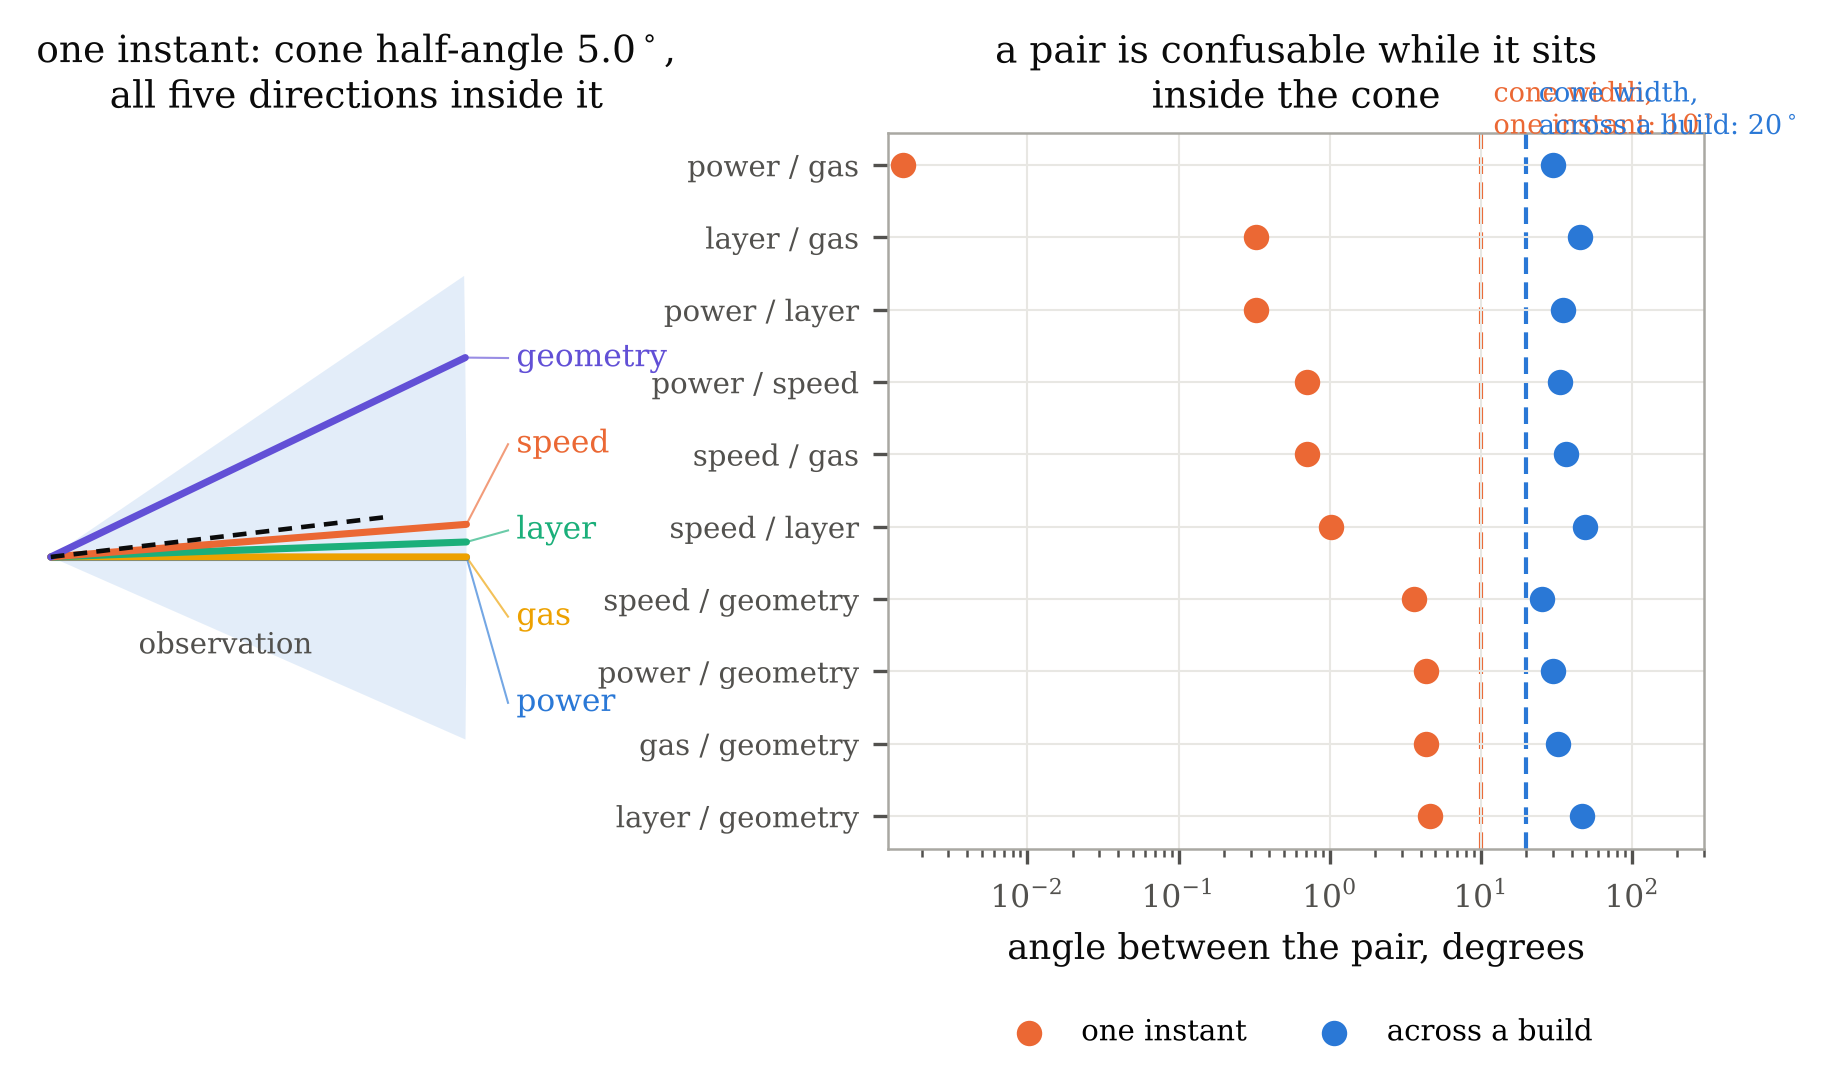
\includegraphics[width=\linewidth]{fig1_cone.png}
\caption{The certificate is a cone about the observation. Each fault's signature
direction is laid out at its true whitened angle from the power direction, and
the shaded wedge is the admissible cone at $\rho = 28$. Reading one instant, the
cone is wider than the spread of directions, so nearly every cause is
admissible; reading across a build, the directions are far enough apart that the
cone isolates one.}
\label{fig:cone}
\end{figure}

\begin{figure}[htbp]
\centering
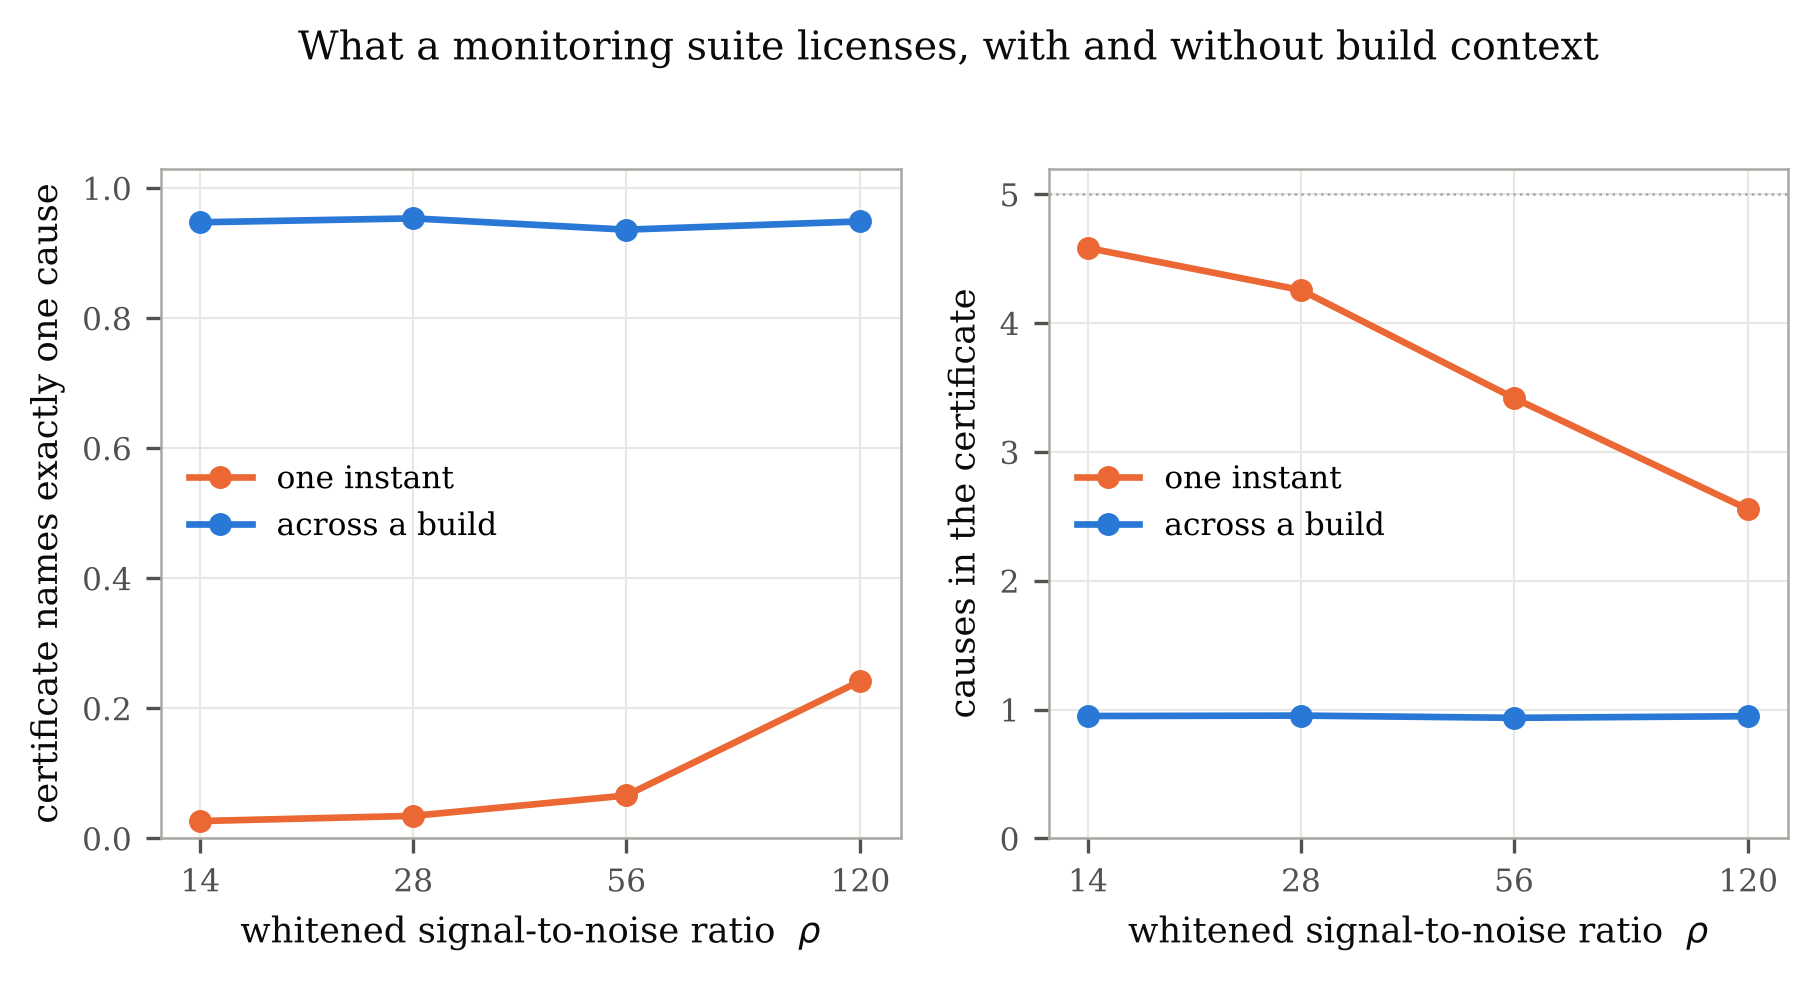
\includegraphics[width=\linewidth]{fig2_certificate.png}
\caption{How often the data licenses naming a single cause, and how many causes
the certificate holds, against whitened signal-to-noise ratio.}
\label{fig:certificate}
\end{figure}

\begin{figure}[htbp]
\centering
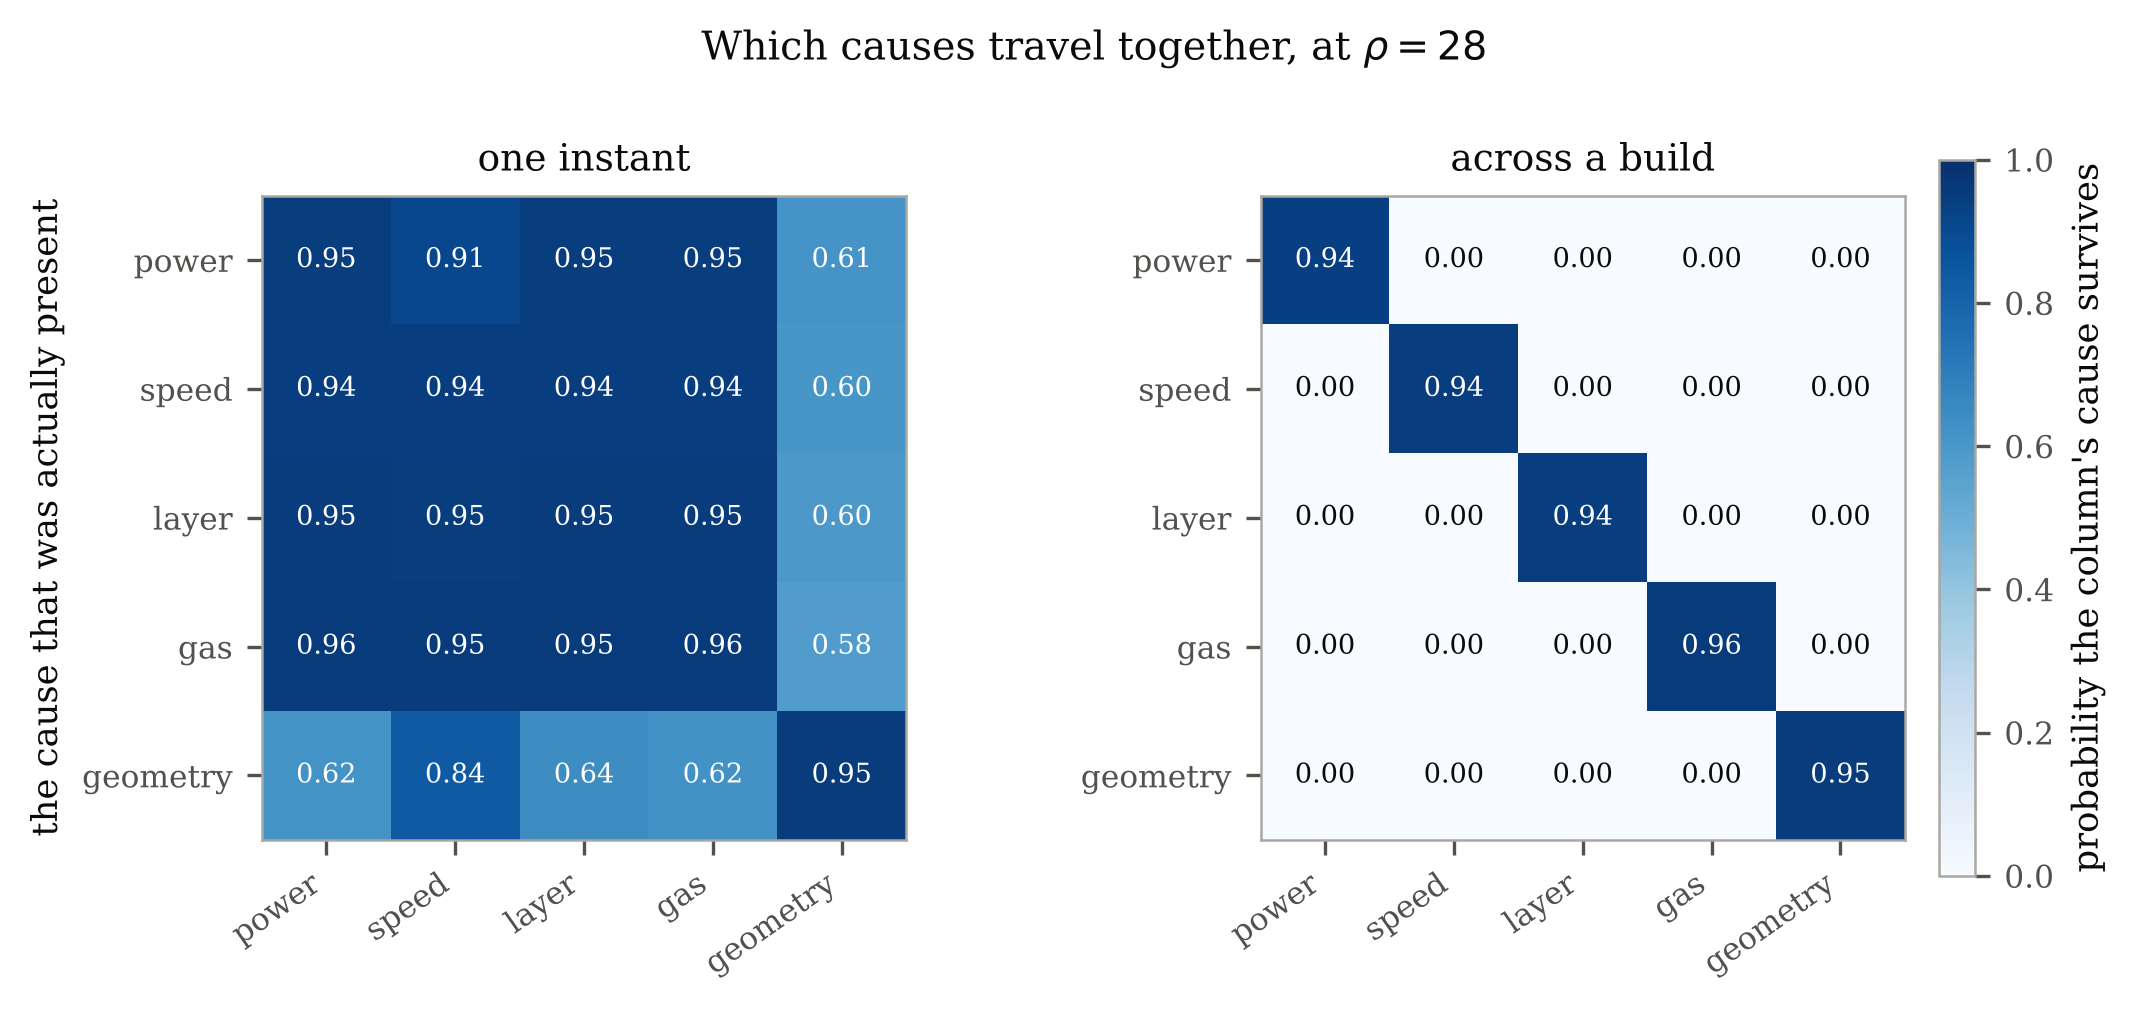
\includegraphics[width=\linewidth]{fig3_admissibility.png}
\caption{The admissibility matrix at $\rho = 28$: the probability that the
column's cause survives a build whose actual cause was the row's. The diagonal
is the coverage and is fixed at $1-\alpha$ by construction.}
\label{fig:admissibility}
\end{figure}

\begin{figure}[htbp]
\centering
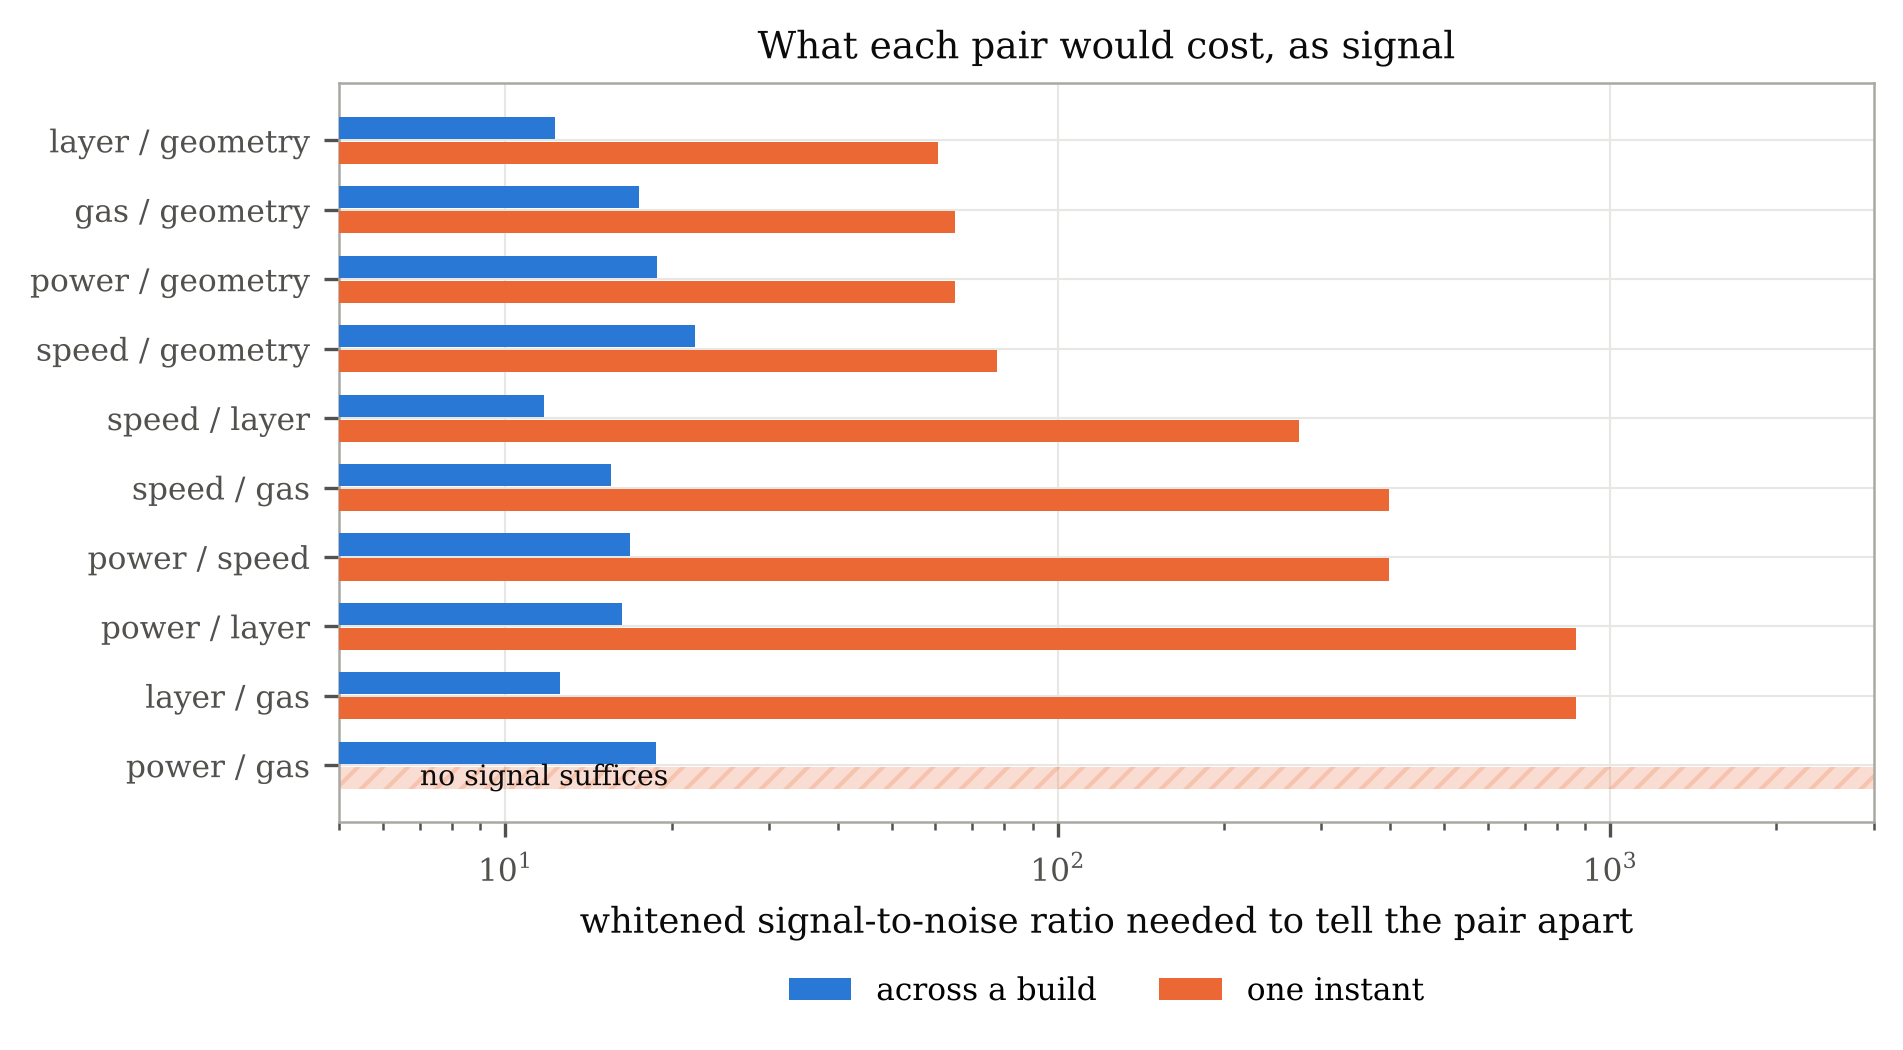
\includegraphics[width=0.85\linewidth]{fig4_required.png}
\caption{The whitened signal-to-noise ratio each pair would need before it stops
being confusable, from Equation~\eqref{eq:floor}. Power against gas is hatched
because no finite signal suffices.}
\label{fig:required}
\end{figure}

\begin{figure}[htbp]
\centering
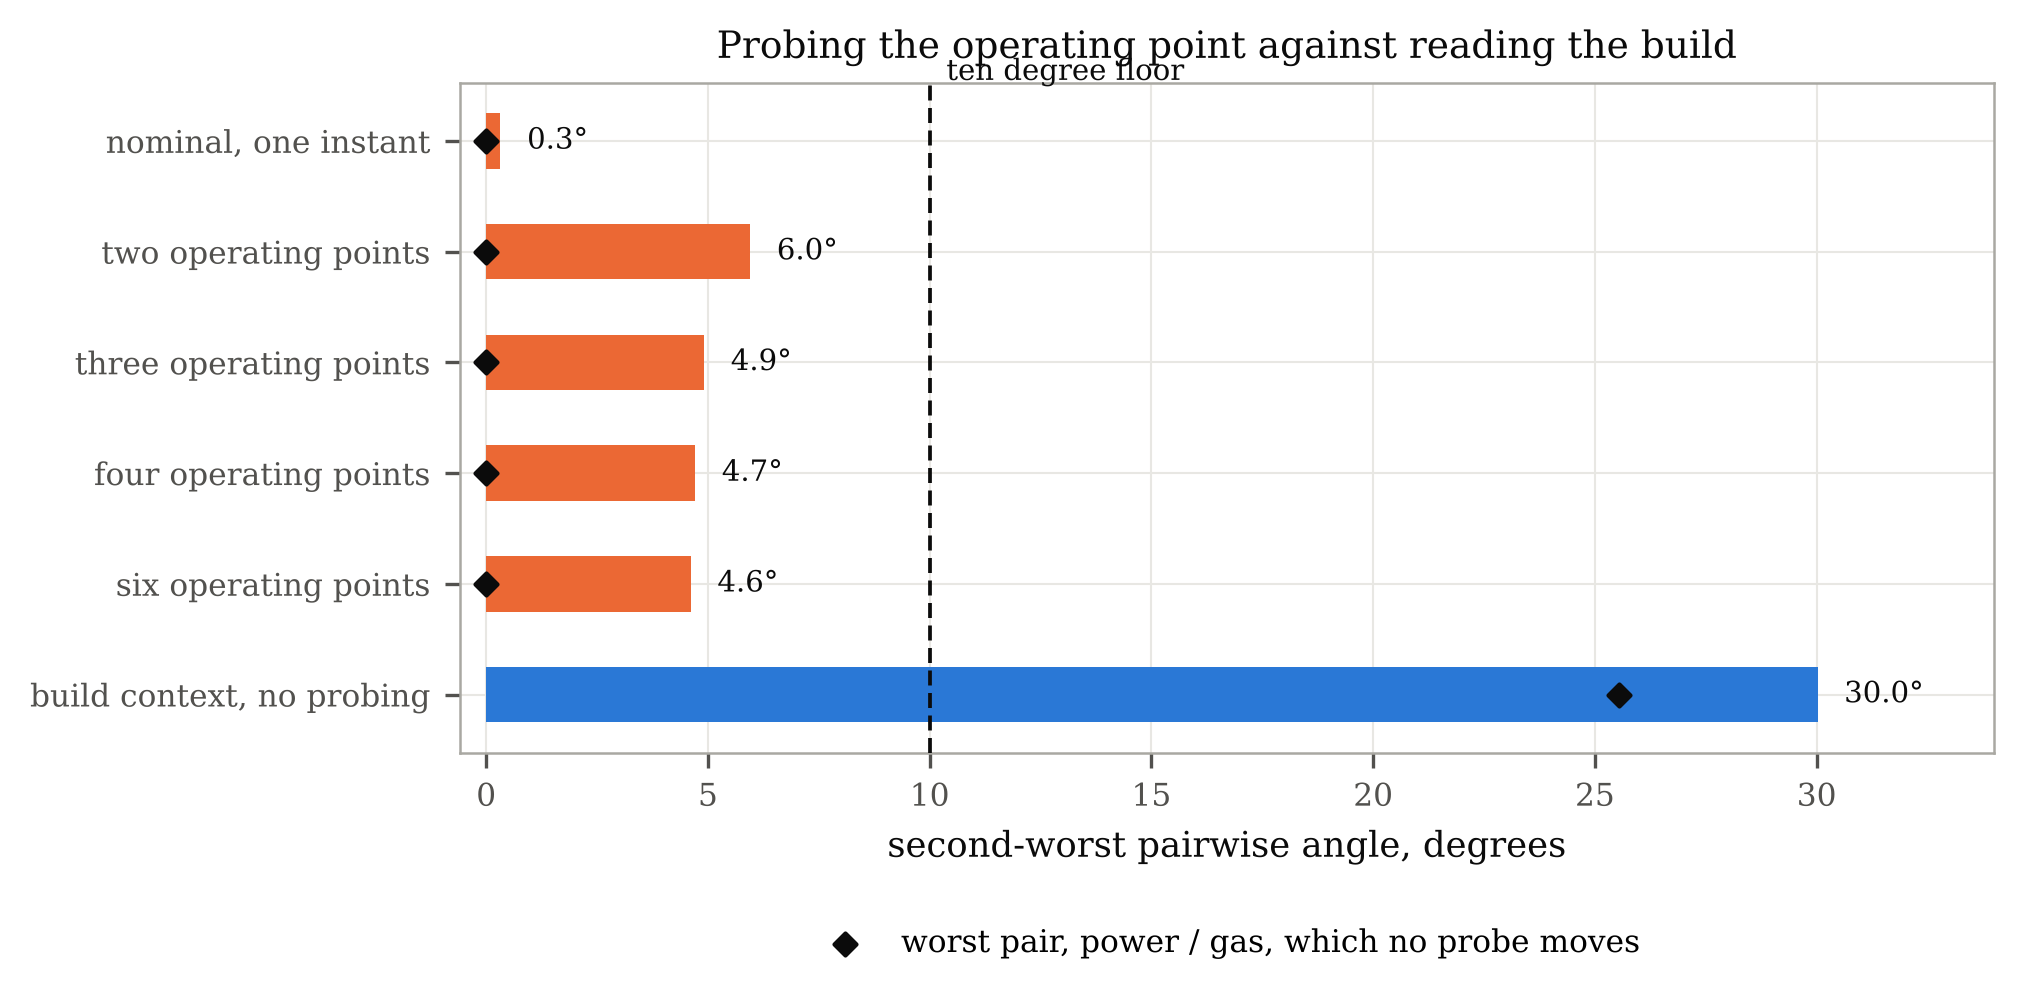
\includegraphics[width=0.85\linewidth]{fig5_probing.png}
\caption{Deliberate probes at further operating points against reading structure
the machine already records. The bar is the second-worst pairwise angle; the
tick is the worst pair, which no probe moves.}
\label{fig:probing}
\end{figure}

\begin{figure}[htbp]
\centering
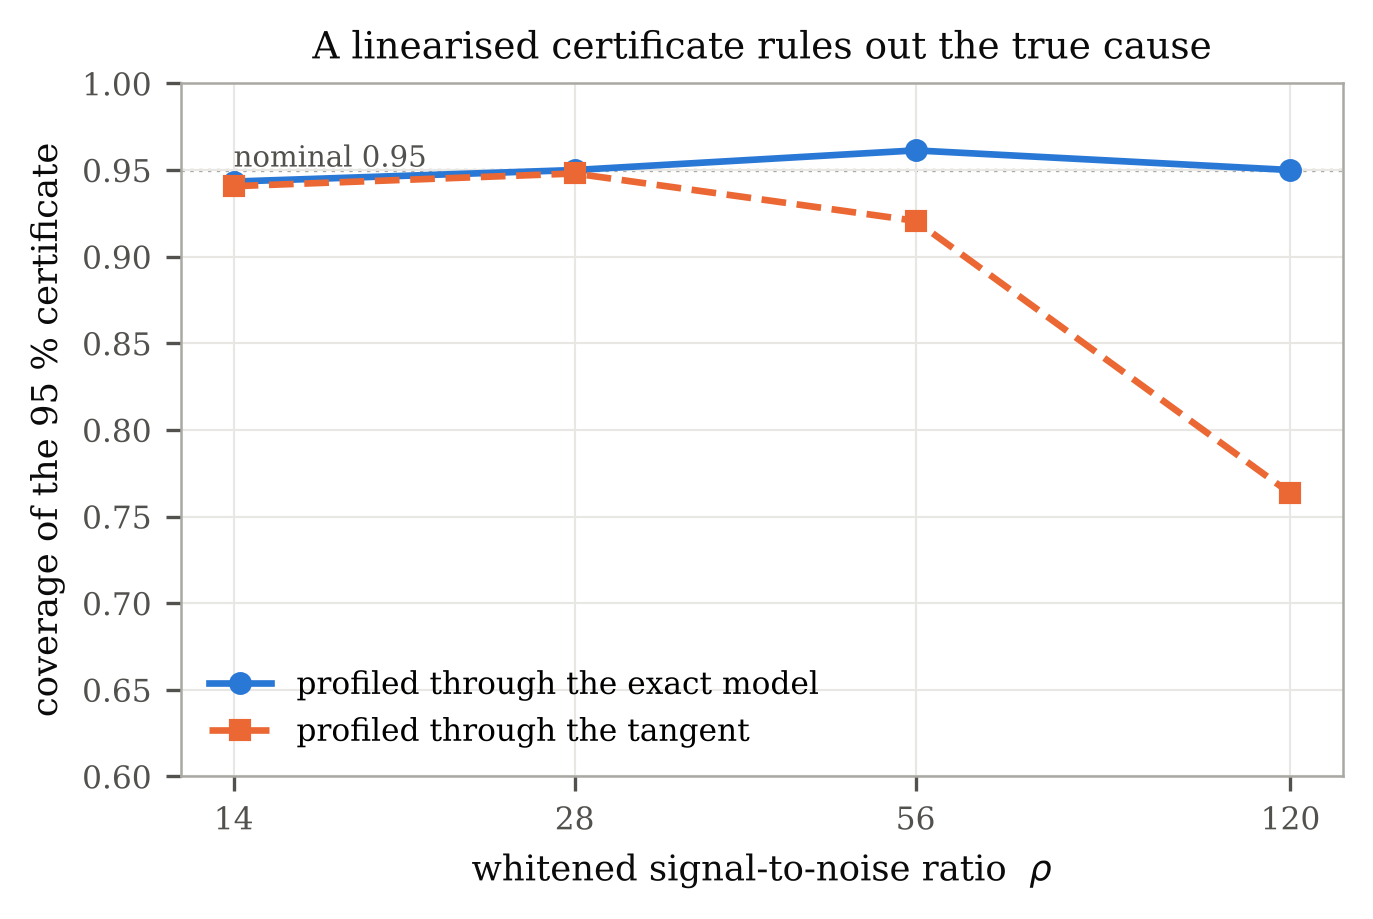
\includegraphics[width=0.7\linewidth]{fig6_coverage.png}
\caption{Coverage of the nominally 95\,\% certificate when the magnitude is
profiled through the exact forward model and when it is profiled through the
model's tangent at the healthy point.}
\label{fig:coverage}
\end{figure}

\end{document}
